\documentclass{article}
\usepackage{cmap}
\usepackage[utf8]{inputenc}
\usepackage[english,ukrainian]{babel}
\usepackage{graphicx}
\usepackage{geometry}
\usepackage{listings}
\usepackage{float}
\geometry{
	a4paper,
	left=20mm,
	right=20mm,
	top=20mm,
	bottom=20mm
}
\lstset{
	language=c,
	tabsize=4,
	keepspaces,
	showstringspaces=false,
}
\graphicspath{ {./pictures} }
\setlength{\parindent}{4em}

\newcommand\subject{Алгоритми та структури даних}
\newcommand\lecturer{доцент кафедри ПЗ\\Коротєєва Т.О.}
\newcommand\teacher{асистент кафедри ПЗ\\Франко А.В.}
\newcommand\mygroup{ПЗ-22}
\newcommand\lab{7}
\newcommand\theme{ }
\newcommand\purpose{}

\begin{document}
	\begin{normalsize}
		\begin{titlepage}
			\thispagestyle{empty}
			\begin{center}
				\textbf{МІНІСТЕРСТВО ОСВІТИ І НАУКИ УКРАЇНИ\\
					НАЦІОНАЛЬНИЙ УНІВЕРСИТЕТ "ЛЬВІВСЬКА ПОЛІТЕХНІКА"}
			\end{center}
			\begin{flushright}
				Інститут \textbf{КНІТ}\\
				Кафедра \textbf{ПЗ}
			\end{flushright}
			\vspace{200pt}
			\begin{center}
				\textbf{ЗВІТ}\\
				\vspace{10pt}
				До лабораторної роботи № \lab\\
				\textbf{На тему}: “\textit{\theme}”\\
				\textbf{З дисципліни}: “\subject”
			\end{center}
			\vspace{112pt}
			\begin{flushright}
				
				\textbf{Лектор}:\\
				\lecturer\\
				\vspace{28pt}
				\textbf{Виконав}:\\
				
				студент групи \mygroup\\
				Коваленко Д.М.\\
				\vspace{28pt}
				\textbf{Прийняв}:\\
				
				\teacher\\
				
				\vspace{28pt}
				«\rule{1cm}{0.15mm}» \rule{1.5cm}{0.15mm} 2022 р.\\
				$\sum$ = \rule{1cm}{0.15mm}……………\\
				
			\end{flushright}
			\vspace{\fill}
			\begin{center}
				\textbf{Львів — 2022}
			\end{center}
		\end{titlepage}
		
		\begin{description}
			\item[Тема.] \theme.
			\item[Мета.] \purpose.
		\end{description}
		
		\section*{Лабораторне завдання}

		\begin{center}

		\end{center}
		
		\section*{Теоретичні відомості}
		
		\section*{Хід роботи}
		\begin{enumerate}
			\item [1024] bubble sort - 1.96ms\\
			selection sort - 473.66µs\\
			shell sort - 83.88µs\\
			quick sort - 46.72µs\\
			merge sort - 112.93µs\\
			counting sort (0..1000) - 10.48µs \\
			counting sort (0..100000) - 186.90µs\\
			counting sort (0..10000000) - 9.84ms \\
			counting sort (0..1000000000) - 938.93ms
			\item [4096] bubble sort - 38.91ms\\
			selection sort - 6.92ms\\
			shell sort - 557.47µs\\
			quick sort - 210.99µs\\
			merge sort - 392.51µs\\
			counting sort (0..1000) - 17.04µs\\
			counting sort (0..100000) - 174.53µs\\
			counting sort (0..10000000) - 12.38ms\\
			counting sort (0..1000000000) - 905.05ms
			\item [16384] bubble sort - 163.02ms\\
			selection sort - 107.53ms\\
			shell sort - 3.23ms\\
			quick sort - 912.83µs\\
			merge sort - 1.62ms\\
			counting sort (0..1000) - 38.27µs\\
			counting sort (0..100000) - 228.31µs\\
			counting sort (0..10000000) - 17.26ms\\
			counting sort (0..1000000000) - 920.33ms
			\item [65536] bubble sort - 6.08s\\
			selection sort - 1.72s\\
			shell sort - 23.23ms\\
			quick sort - 4.09ms\\
			merge sort - 7.11ms\\
			counting sort (0..1000) - 122.78µs\\
			counting sort (0..100000) - 762.67µs\\
			counting sort (0..10000000) - 20.39ms\\
			counting sort (0..1000000000) - 968.31ms
			\item [262144] bubble sort - 50.35s\\
			selection sort - 26.93s\\
			shell sort - 227.47ms\\
			quick sort - 17.64ms\\
			merge sort - 28.93ms\\
			counting sort (0..1000) - 475.76µs\\
			counting sort (0..100000) - 1.38ms\\
			counting sort (0..10000000) - 24.02ms\\
			counting sort (0..1000000000) - 1.16s
			\item [1048576] bubble sort - timeout\\
			selection sort - 432.64s\\
			shell sort - 1.92s\\
			quick sort - 78.55ms\\
			merge sort - 122.68ms\\
			counting sort (0..1000) - 3.78ms\\
			counting sort (0..100000) - 4.13ms\\
			counting sort (0..10000000) - 38.42ms\\
			counting sort (0..1000000000) - 1.65s
			\item [4194304] bubble sort - timeout\\
			selection sort - timeout\\
			shell sort - 13.94s\\
			quick sort - 341.88ms\\
			merge sort - 520.15ms\\
			counting sort (0..1000) - 11.44ms\\
			counting sort (0..100000) - 14.85ms\\
			counting sort (0..10000000) - 97.69ms\\
			counting sort (0..1000000000) - 2.16s
		\end{enumerate}
		
		\begin{figure}[H]
			\centering
			\includegraphics[scale=0.5]{1}	
			\caption{Графік}
		\end{figure}
	
		\begin{figure}[H]
			\centering
			\includegraphics[scale=0.5]{2}	
			\caption{Графік}
		\end{figure}
		
		\begin{figure}[H]
			\centering
			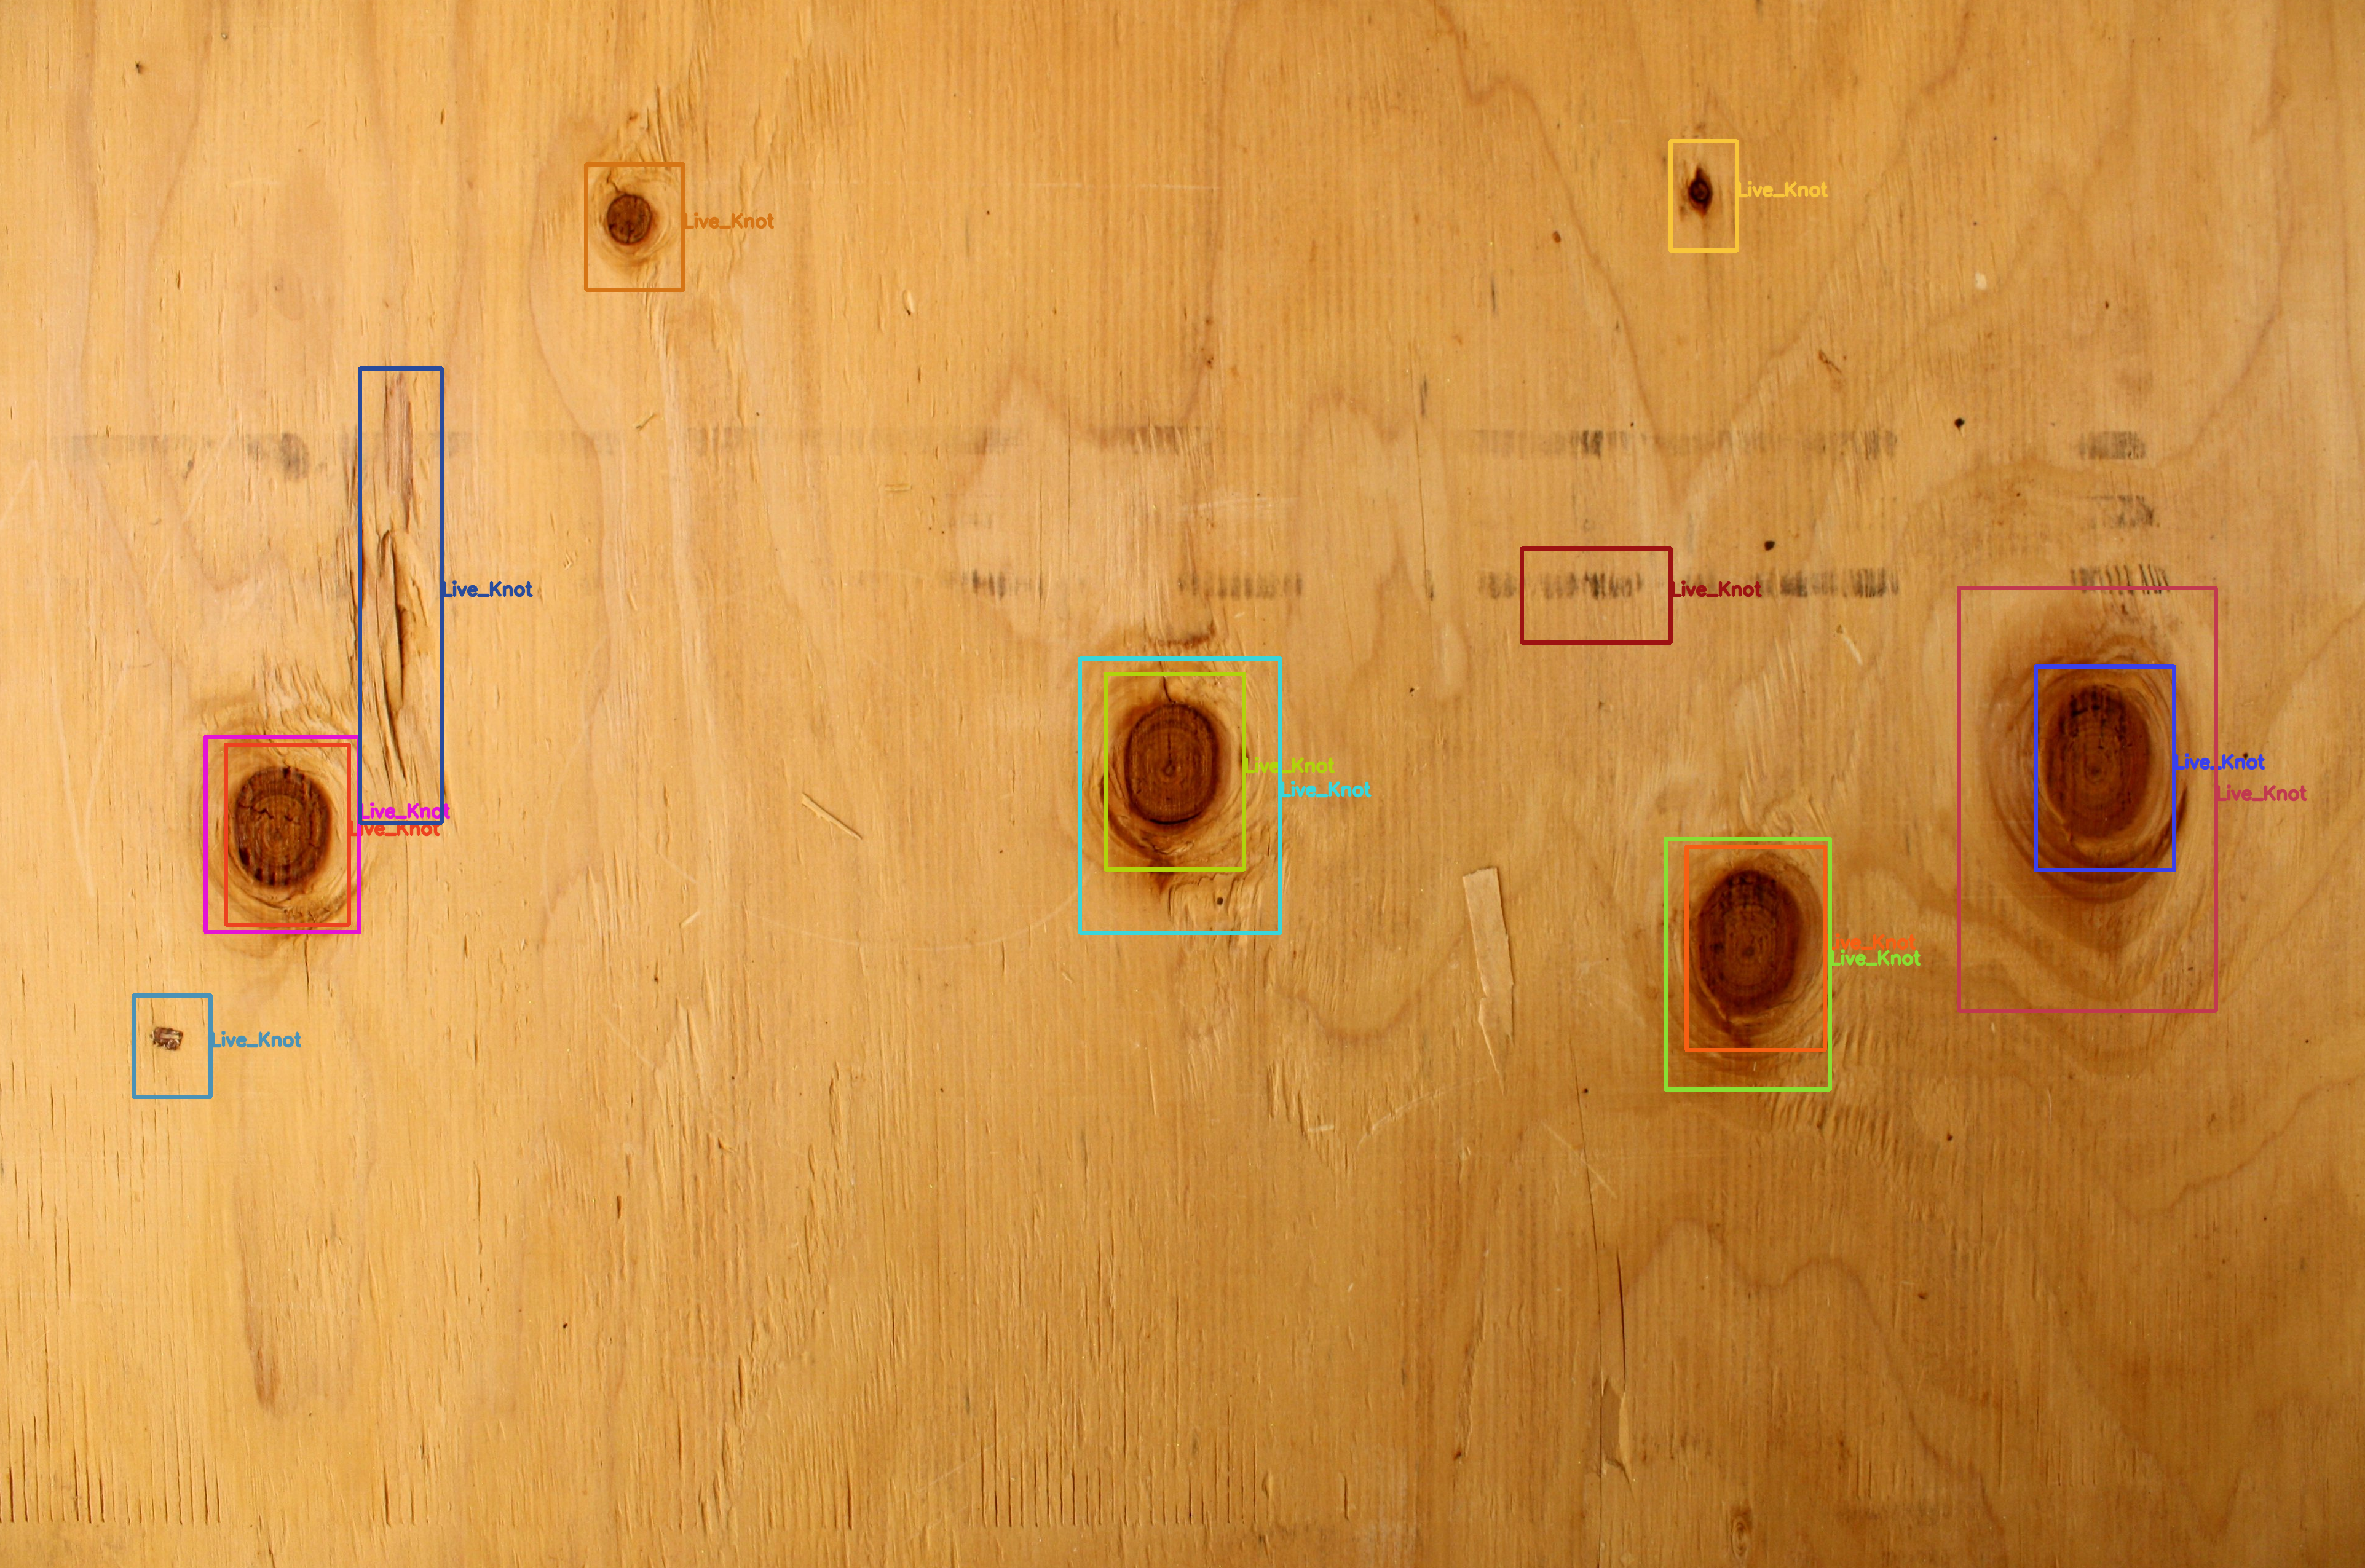
\includegraphics[scale=0.5]{3}	
			\caption{Графік}
		\end{figure}
		
		\section*{Висновок}
		
		
	\end{normalsize}
\end{document}
